\documentclass[dvipdfmx, 9pt, a4paper]{jsarticle}
\usepackage[margin=15mm]{geometry}
\usepackage{fancyhdr}
\usepackage{multirow}
\usepackage{amsmath,  amssymb}
\usepackage{type1cm}
\usepackage{latexsym}
\usepackage{algorithmic}
\usepackage{algorithm}
\usepackage{ascmac}
\usepackage{listings,jvlisting}
\usepackage{tcolorbox}
\usepackage[utf8]{inputenc}
\usepackage{color}

\DeclareFixedFont{\ttb}{T1}{txtt}{bx}{n}{9}
\DeclareFixedFont{\ttm}{T1}{txtt}{m}{n}{9}
\definecolor{deepblue}{rgb}{0,0,0.5}
\definecolor{deepred}{rgb}{0.6,0,0}
\definecolor{deepgreen}{rgb}{0,0.5,0}

\renewcommand{\baselinestretch}{0.78}
\newcommand{\bm}[1]{{\mbox{\boldmath $#1$}}}
\newtheorem{Proof}{証明}
\def\qed{\hfill $\Box$}

\newcommand\pythonstyle{\lstset{
language=Python,
basicstyle=\ttm,
morekeywords={self},
keywordstyle=\ttb\color{deepblue},
emph={MyClass,__init__},
emphstyle=\ttb\color{deepred},
stringstyle=\color{deepgreen},
frame=tb,
showstringspaces=false
}}

\lstnewenvironment{python}[1][]
{
\pythonstyle
\lstset{#1}
}
{}

\newcommand\pythonexternal[2][]{{
\pythonstyle
\lstinputlisting[#1]{#2}}}
\newcommand\pythoninline[1]{{\pythonstyle\lstinline!#1!}}


\begin{document}
\begin{center}
{\fontsize{18pt}{1pt}\selectfont 最適輸送}\\
\end{center}

\section*{はじめに}
最適輸送と聞けば巡回セールスマン問題のようなものを想像されるかもしれないが、本資料で扱うものはそれと異なる。本資料でいう最適輸送とは確率分布と確率分布、もしくは点群と点群を比較する学問を指す。確率分布の比較として有名なものにKLダイバージェンスがあるが、その限りではない。エンジニアは様々な比較手法の中から、問題に適した一つを選択しなければならない。その素質を身につけるために本資料を執筆することにした。本資料では下記3種の確率分布の比較を取り扱う。
\begin{figure}[b]
\begin{center}
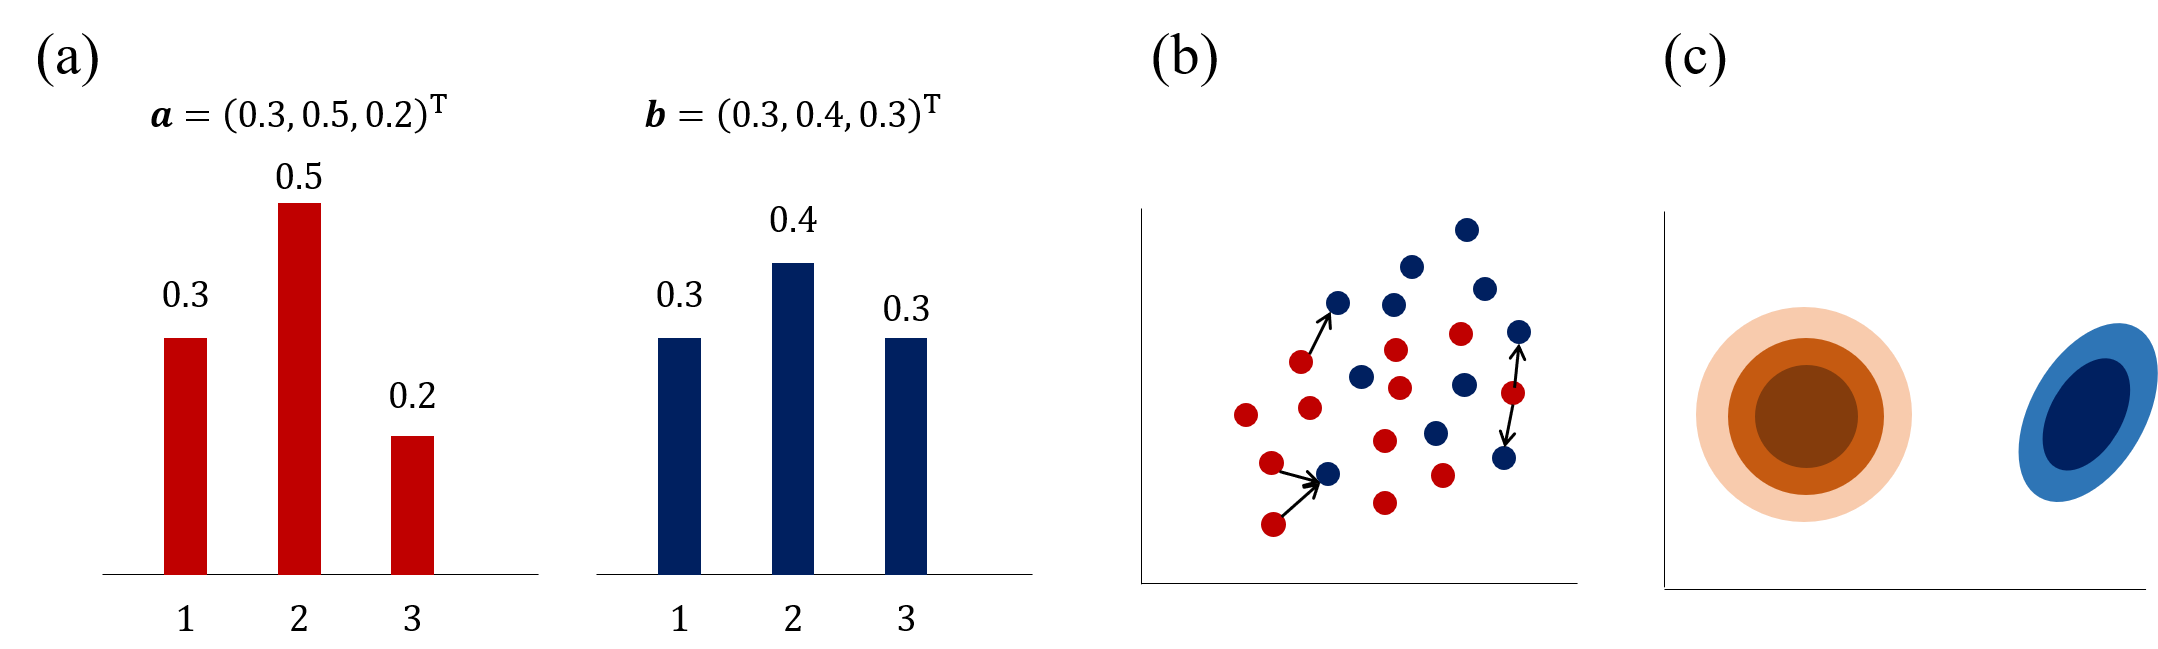
\includegraphics[width=16cm]{fig1.png}
\caption{確率分布の比較例。(a)ヒストグラムの比較(b)点群比較(c)連続確率分布の比較。}
\end{center}
\end{figure}

\begin{itemize}
\item {\bf ヒストグラムの比較}\\
本資料におけるヒストグラムとは有限離散カテゴリ上の確率分布のことを指す。例えば\{犬:0.2, 猫:0.5, 鳥:0.3\}のようにカテゴリ毎に確率値が与えられている場合、これは確率分布を成していると言える。カテゴリ数を$n$、各カテゴリ$i$に対応する確率値を$a_i(i \in [n])$としたとき、確率分布は$n$次元の数ベクトル$\bm a=(a_1, ..., a_n)^{\rm T}$で表される。なお、確率の公理より$a_i \geq 0(i \in [n])$及び$\sum_i a_i=1$が成り立つが、このような数ベクトルを確率ベクトルと言う。\par
確率分布の比較とはベクトル$\bm a$と$\bm b$の比較に帰着する。より感覚的は、「$\bm a$を$\bm b$に一致させるためには、$a_i$間で少なくともどれ程の値の調整をしなければならないか」と言える。例えば図1(a)のベクトル$\bm a$と$\bm b$を考える。$\bm a$を$\bm b$に一致させるには$a_2$のうち0.1だけを$a_3$に輸送すればよい。もちろん、$a_1$から0.1を$a_2$に送り、$a_2$から0.1を$a_3$に送り、更に$a_3$から0.1を$a_1$に送っても、その結果は$\bm b$と一致する。しかしながら、その輸送に要するコストのようなものは明らかに前者と比べて大きい。当然ながら最小コストの値で測ることが確率分布の比較として妥当である。各確率$a_i$を質量と捉え、各カテゴリ$i$に運搬するのに要するコストと例えることもできるので、最適輸送のことを土砂運搬距離と呼ぶこともある。
\item {\bf 点群比較}\\
ユークリッド空間に埋め込まれた有限サイズの離散分布を、本資料では点群と呼ぶ(図1(a))。一般的に点群は同じ重み、確率値を与える。点群の総数を$n$としたとき、点群全体は$\sum_i \delta(\bm x - \bm x_i)/n$なる確率分布を表していると考えてもよい。未知の確率分布$p(\bm x)$からサンプリングされた結果得られたものという意味で、この確率分布は経験分布と呼ばれている。\par
確率分布の比較とは経験分布の比較に帰着する。今回の場合、各点に$1/n$の質量がある訳で、それを図1(b)のように運搬するするときの土砂運搬距離が所望の測度である。図1(b)にある通り、$1/n$の質量を分割して異なる点に運搬してもよいし、質量を受け取る側も複数の点から供給されてもよい。
\item {\bf 連続確率分布の比較}\\
考え得る比較の最後は連続確率分布同士の比較である(図1(c))。例えば二つの正規分布の比較などが考えられる。単純な確率分布であれば解析的に比較することができるが、それができない確率分布も存在する。対策案として、対象の確率分布からいくつかサンプリングし、点群の比較に置き換えることが考えられる。
\end{itemize}\par
KLダイバージェンスは確率分布の比較に関する測度だが、本資料で扱う最適輸送には属さない。最適輸送はKLダイバージェンスにない特性を有しており、その分機械学習などで有益であると言われている。そのことを理解するためにまずはKLダイバージェンスについて復習しよう。まずは確率ベクトルに対するKLダイバージェンスである。
\begin{tcolorbox}[title=確率ベクトルに対するKLダイバージェンス]
 2つの確率ベクトル$\bm a$、$\bm b \in \mathbb{R}^n$を考える。確率ベクトルに対するKLダイバージェンスは下記のように定義される(ただし0log0=0)。
\begin{equation}
{\rm KL}(\bm a||\bm b)=\sum_{i=1}^n\left(a_i{\rm log}\frac{a_i}{b_i}-a_i+b_i\right)
\end{equation}
\end{tcolorbox}
KLダイバージェンスが大きいほど両確率分布は異なる。特に、ある$i \in [n]$において$a_i>0$かつ$b_i=0$であるとき、KLダイバージェンスは$\infty$となる。なお、$\sum(-a_i+b_i)=0$であるため右辺第一項以外は結果に影響を与えないが、技術的な都合上この項を含める形で定義する。\par
次に連続な確率分布におけるKLダイバージェンスを紹介する。
\begin{tcolorbox}[title=確率密度関数に対するKLダイバージェンス]
 確率変数の集合を$X$とし、2つの確率密度関数$p, q:X \to \mathbb{R}$を考える。このときKLダイバージェンスは以下の通りである(ただし$0\log0=0$)。
\begin{equation}
{\rm KL}(p||q)=\int_X\left( p(x)\log\left(\frac{p(x)}{q(x)}\right)-p(x)+q(x) \right)
\end{equation}
\end{tcolorbox}
KLダイバージェンスの値が大きいほど両確率密度関数は異なる。特に、$p(x)>0$かつ$q(x)=0$となる$x \in X$が存在するとき、KLダイバージェンスは$\infty$となる。\par
KLダイバージェンスには以下のような問題が指摘されている。
\begin{itemize}
\item {\bf 距離構造を捉えられない}:例えば翌日の気温を予測するクラス分類器を考える(本来なら回帰モデルを使う所だが、説明のためクラス分類器で考えることにする)。このクラス分類器は$X=\{21, 22, 23, 24, 25, 26\}$に関する確率ベクトルを出力するとしよう。図2は教師データ(図中A)と異なる2つの予測結果(B, C)を表したヒストグラムである。BとCは異なるクラス分類器から出力されたもので、どちらが優れているかを判断したい。そこで、Aの確率ベクトルとの類似度を測る訳だが、KLダイバージェンスを測度にした場合、BとCはAと同じだけ類似していることになる。しかしながら、22が最頻値であるAに対し、最頻値が23にあるBの方がCよりも優れていると直感的には考えるだろう。KLダイバージェンスは土砂運搬距離のような考え方ができず、BとCに優劣はないと判断してしまう。
\item {\bf サポートが一致していないと定義できない}:集合$X$のうち、確率値が正の部分集合のことをサポートと言う。KLダイバージェンスは両確率分布のサポートが一致していないと定義できない。例えば前述したように、式(1)に関して$a_i>0$かつ$b_i=0$を満たすような$i$が存在するとき、KLダイバージェンスに$-a_i\log0$の項が現れKLダイバージェンスは$\infty$となる。
\end{itemize}

\begin{figure}[b]
\begin{center}
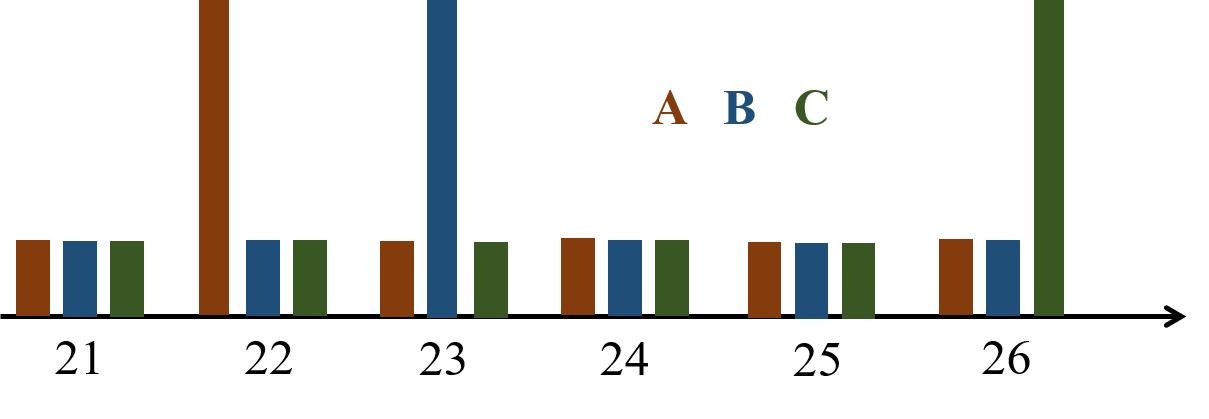
\includegraphics[width=12cm]{fig2.png}
\caption{KLダイバージェンスが距離構造を捉えられない例。}
\end{center}
\end{figure}

本資料で取り扱う最適輸送はこういった問題を回避してくれる。次章では最適輸送を定式化していく。

\section{最適化問題としての定式化}
\subsection{線形計画による定式化}
本節では最適輸送問題を線形計画問題として定式化する。このときの決定変数は輸送方法であり、目的関数は輸送コストとなる。したがってさいてきゆ問題は輸送コストの最適化と言える。
\subsubsection{点群の比較}
集合$V$上で定義された点群を考える。いま2つの点群の部分集合$X=\{\bm x_1, ..., \bm x_n|\bm x_i \in V\}$、$Y=\{\bm y_1, ..., \bm y_n|\bm y_i \in V\}$が与えられたとする。本問題では、$X$と$Y$の最小輸送コストを求め、それを基にして両部分集合の類似度を評価する。\par
集合$V$上の各対$\bm a, \bm b \in V$に対して$\bm a$から$\bm b$への輸送コスト$C(\bm x, \bm y)$が与えられているとする。この関数$C:V \times V \to \mathbb{R}$のことをコスト関数と言う。$C(\bm a, \bm b)$は負であっても構わないが、実際の問題では非負とすることが多い。例えばユークリッドノルム$C(\bm a, \bm b)=||\bm a-\bm b||_2$などが考えられる。\par
$X$に関して点$\bm x_i$の重みを$x_i$とし、ベクトル$\bm x=(x_1, ..., x_n)^{\rm T}$と表すことにする。同様に$Y$に関して点$\bm y_i$の重みを$y_i$とし、ベクトル$\bm y=(y_1, ..., y_m)^{\rm T}$のように表す。なお、$\bm x$と$\bm y$の次元は$n$と$m$であり、同じである必要はない。また、$n=m$の場合であっても、それぞれの基底の意味する所は異なる。\par
点$\bm x_i$から$\bm y_j$へ輸送される質量を$P_{ij}$とする。$P_{ij}$は以下の制約を満たす。
\begin{equation}
P_{ij} \geq 0,~~~\sum_i P_{ij}=y_j,~~~\sum_j P_{ij}=x_i \notag
\end{equation}
上式のうち後半2つの制約は質量保存制約と呼ばれている。\par
各対$(i, j)$を纏めた行列$P\in \mathbb{R}^{n\times m}$を輸送行列という。最適輸送問題は輸送コストを最小にする輸送行列の決定と言うことができる。コスト関数が与えられているとき、輸送行列$P$に対応する輸送コストは
\begin{equation}
\sum_i^n\sum_j^mC(\bm x_i, \bm y_j)P_{ij} \notag
\end{equation}
より求められる。この最小値を最適輸送コストと呼び、${\rm OT}(\bm x, \bm y, C)$と書き表す。\par
$P_{ij}$を成分に持つ行列$P \in \mathbb{R}^{n \times m}$のことを輸送行列と言う。輸送行列を用いれば、質量保存制約を$P\mathbb{I}_m=\bm x$、$\mathbb{I}_nP=\bm y$のように書き換えることもできる(ここで$\mathbb{I}_m$は全ての成分が1の$m$次元ベクトル)。制約条件を満たす輸送行列全体の集合$\{P|P_{ij} \geq 0,~~P\mathbb{I}_m=\bm x,~~\mathbb{I}_nP=\bm y\}$(つまり最適輸送問題の実行可能領域)を$\mathcal{U}(\bm x, \bm y)$と書き、輸送多面体と呼ぶ。ここで$\tilde{P}=\bm x\bm y^{\rm T} \in \mathbb{R}^{n \times m}$は、明らかに制約を満たすので、輸送多面体は空集合でない。\par
$C_{ij}=C(\bm x_i, \bm y_j)$を成分にもつ行列$C \in \mathbb{R}^{n \times m}$のことをコスト行列と言う。いま、行列の内積$\mathbb{R}^{n \times m}\times \mathbb{R}^{n \times m} \to \mathbb{R}$を$<A, B>=\sum_{ij}A_{ij}B_{ij}$としたとき、最適輸送コストは${\rm OT}(\bm x, \bm y, C)={\rm min}_{P \in \mathcal{U}(\bm x, \bm y)}<C, P>$となる。目的関数と制約が線形であるため、この問題は線形計画問題に分類される。また、この定式化をカントロヴィチの定式化と言う。
\begin{tcolorbox}[title=カントロヴィチの定式化]
点群$X=\{\bm x_1, ..., \bm x_n\}$の各点$\bm x_i$の重みを$x_i$とし、ベクトル$\bm x=(x_1, ..., x_n)^{\rm T}$で纏める。同様に点群$Y=\{\bm y_1, ..., \bm y_m\}$の各点$\bm y_i$の重みを$y_i$とし、ベクトル$\bm y=(y_1, ..., y_m)^{\rm T}$で纏める。またコスト行列を$C \in \mathbb{R}^{n \times m}$とする。カントロヴィチの定式化では、
\begin{equation}
{\rm min}_{P \in \mathcal{U}(\bm x, \bm y)}<C, P>
\end{equation}
の$n$行$m$列行列$P$を求める。ここで、$\mathcal{U}(\bm x, \bm y)=\{P|P_{ij} \geq 0,~~P\mathbb{I}_m=\bm x,~~\mathbb{I}_nP=\bm y\}$である。
\end{tcolorbox}\par
以下にPythonコード例を示す。例題として
\begin{equation}
\begin{array}{llll}
\bm x_1 = (2.2, 2.1)^{\rm T}&\bm x_2 = (3.2, 5.3)^{\rm T}&\bm x_3 = (4.5, 4.4)^{\rm T}&\bm x_4 = (3.1, 3.8)^{\rm T} \\
\bm y_1 = (4.8, 1.9)^{\rm T}&\bm y_2 = (4.1, 3.3)^{\rm T}&\bm y_3 = (2.0, 5.5)^{\rm T}&\bm y_4 = (3.4, 2.5)^{\rm T} 
\end{array}\notag
\end{equation}
に位置する点群を考える。また、各点の重みは等しく$1/4$とした。コスト関数はL2ノルムの2乗とする。線形計画問題はscipyのシンプレックス法で解いた。ただしscipyのシンプレックス法の目的関数はベクトルの内積で表現されているため、コスト行列や輸送行列も関数内ではベクトルで定義している。線形計画問題が解けてから、輸送ベクトルを行列に定義し直して出力する。
\begin{python}
import numpy as np
from scipy.optimize import linprog

def Kantorovich(C, a, b):
	c = C.flatten()
	Aeq = []

	for i in range(len(a)):
		aeq = np.zeros(C.shape)
		aeq[i,:] = 1.
		Aeq.append(aeq.flatten())

	for j in range(len(b)):
		beq = np.zeros(C.shape)
		beq[:,j] = 1.
		Aeq.append(beq.flatten())

	Aeq = np.stack(Aeq, axis = 0)
	beq = np.concatenate((a, b))

	result = linprog(c, A_eq = Aeq, b_eq = beq, method = "simplex")
	P = (result.x).reshape(C.shape)

	return P

X = np.array([
	[2.2, 2.1],
	[3.2, 5.3],
	[4.5, 4.4],
	[3.1, 3.8]])

Y = np.array([
	[4.8, 1.9],
	[4.1, 3.3],
	[2.0, 5.5],
	[3.4, 2.5]])

C = np.zeros((4, 4))
for i in range(4):
	for j in range(4):
		C[i, j] = (np.linalg.norm(X[i] - Y[j])**2)

a = 0.25*np.ones(4)
b = 0.25*np.ones(4)

P = Kantorovich(C, a, b)
\end{python}

\subsubsection{ヒストグラムの比較}
ヒストグラムの比較は点群の比較と同じように定式化できる。それぞれ確率ベクトル$\bm x, \bm y \in \mathbb{R}^n$が与えられ、前節と同様にコスト行列$C \in \mathbb{R}^{n \times n}$が定義される。この問題の目的は最適な輸送行列$P \in \mathbb{R}^{n \times}$を見つけることであり、目的関数や制約条件は以下のように書き表される。
\begin{equation}
{\rm min}_{P \in {\mathcal{U}(\bm x, \bm y)}}<C, P>,~~~\mathcal{U}(\bm x, \bm y)=\{P|P_{ij}\geq 0,~P\mathbb{I}_n=\bm x,~\mathbb{I}_nP=\bm y\} \notag
\end{equation}
これは正にカントロヴィチの定式化である。

\subsubsection{連続確率分布の比較}
確率分布が定義されている確率変数の全ての集合を$\mathcal{X}$と書く。比較対称の確率分布$a(\bm x)$と$b(\bm x)$は当然ながら任意の$\bm x(\in \mathcal{X})$で定義されている。ただし$\bm x$は連続であるため、$a$と$b$の次元は基本的に無限となり、1.1.1や1.1.2のように定式化できない。\par
そこで、確率分布$a$と$b$はそのまま関数として扱い、これまでの輸送行列$P$に相当するものも関数$\pi$として扱う。この$\pi$のことを輸送と言う。定義より、輸送$\pi$は$\mathcal{X}\times \mathcal{X} \to \mathbb{R}$の関数となる。同様に、これまでのコスト行列に相当する関数$C:\mathcal{X}\times \mathcal{X} \to \mathbb{R}$も定義し、これをコスト関数と呼ぶ。このとき、輸送コストは
\begin{equation}
\int_{\mathcal{X}\times \mathcal{X}}C(x, y)\pi(x, y)dxdy \notag
\end{equation}
と定式化される。\par
いま、$a$から$b$への輸送を考えているため、$\pi$の取り得る確率分布にも制約があり、
\begin{equation}
\int_{\mathcal{X}}\pi(x_a, x)dx=a(x_a)~(x_a \in \mathcal{X})~~~\int_{\mathcal{X}}\pi(x, x_b)dx=b(x_b)~(x_b \in \mathcal{X}) \notag
\end{equation}
のように表される。これは正に確率分布の周辺化であり、カントロヴィチの定式化でも見られた。上式の制約に加えて、$\pi(x_a, x_b) \geq 0$の制約も$\pi$は満たさなければならない。
\begin{tcolorbox}[title=確率分布の最適輸送問題]
 確率分布が定義されている確率変数の全ての集合を$\mathcal{X}$と書く。また、$\bm x$に対して確率分布$a(\bm x)$と$b(\bm x)$を考える。コスト関数を$C: \mathcal{X}\times \mathcal{X} \to \mathbb{R}$と定義したとき、最適輸送問題は
\begin{equation}
{\rm min}_{\pi}\int_{\mathcal{X}\times \mathcal{X}}C(x, y)\pi(x, y)dxdy
\end{equation}
の問題として定式化できる(この最適値を${\rm OT}(a, b, C)$と書く)。ここで輸送$\pi$は
\begin{equation}
\int_{\mathcal{X}}\pi(x_a, x)dx=a(x_a)~(x_a \in \mathcal{X})~~~\int_{\mathcal{X}}\pi(x, x_b)dx=b(x_b)~(x_b \in \mathcal{X})~~~\pi(x_a, x_b) \geq 0 \notag
\end{equation}
を満たさなければならない。
\end{tcolorbox}\par
連続確率分布の最適輸送問題も線形問題と言えるが、確率分布の次元が無限であるため、シンプレックス法のような線形計画法で解くことはできない。数値計算をする場合、確率分布から有限個のサンプリングを行い、点群の比較に帰着させるか、この問題の双対問題の決定変数となる連続関数をニューラルネットワークでモデル化して解くといったアプローチが取られる(後述)。

\subsection{ワッサースタイン距離}
最適輸送コストは、その直感的な意味から最適輸送距離と呼ばれることもあるが、必ずしも距離の公理を満たしている訳ではない。例えばコスト関数が$C \equiv 0$である場合、任意の分布間に関して輸送コストはゼロになる。本章で紹介するワッサースタイン距離は輸送コストの特殊例であり、距離の公理を満たすようになっている。

\begin{tcolorbox}[title=ワッサースタイン距離]
 $\mathcal{X}$上の距離関数$d:\mathcal{X}\times \mathcal{X} \to \mathbb{R}$と1以上の実数$p$について、コスト関数を$C(\bm x, \bm y)=d(x, y)^p$と定義する。このとき、確率ベクトルもしくは確率密度関数$a$及び$b$について$OT(a, b, C)^{1/p}$をワッサースタイン距離と言い、$W_p(a, b)$と書く。
\end{tcolorbox}
\begin{itembox}[l]{定理1}
ワッサースタイン距離は距離の公理を満たす。つまり、
\begin{enumerate}
\item $W_p(a, b)=0$のときかつそのときのみ$a=b$。
\item $W_p(a, b) =W_p(b, a)$。
\item $W_p(a, b)+W_p(b, c) \geq W_(a, c)$。
\end{enumerate}
\end{itembox}

\subsection{最適輸送の双対問題}
最適輸送問題は、これまで見てきた最小化問題の双対問題をもとに解かれることが多い。そこで、本節では最適輸送から一旦離れて、双対問題自体について議論していく。\par
まず、最小化問題の実行可能解$P$が手に入ったとし、その目的関数値$L(P)$が80.0だったとする。この解がどれ程良いかは当然ながら最適値次第であろう。つまり、もし最適値が$L(P^*)=79.9$であれば$P$は最適値に迫る良い解だと言えるし、逆に$L(P^*)=20.0$であればまだまだ改善の余地ありだと言える。仮に手元にある実行可能解が良い解だと分かれば、これ以上の改善を打ち切って近似解とすることもできる。しかし、最後まで最適化問題を解かなければ最適解が分からない点が厄介であり、そもそも解の良さが評価できるなら最適解は所与である状況にあると言える。\par
そこで、今解きたい問題よりも最適値が小さく、かつ簡単に解ける代替問題を考える。この問題を解いた結果、最適値が79.8だと分かったとしよう。すると、今解きたい最適化問題の最適値は79,8以上であることが保証されるので、$L(P)=80.0$は良い解だと言える。このように現段階の解を評価するための代替問題を双対問題と言う。\par
双対問題の最適値は解きたい問題の最適値に近くなければならない。例えば元の問題の最適値が79.9であるのに対し、双対問題の最適値が20.0であったとする。この場合、$L(P)=80.0$という結果は改善の予知があるのか否かが判断できない。
\subsubsection{ラグランジュの未定乗数法}
双対問題の代表的な例にラグランジュの未定乗数法がある。例えば
\begin{equation}
{\rm min}_{\bm x}f(x)~~~{\rm s.t.}~~h_i(\bm x) \leq 0~(i=1, ..., n)~~h_i(\bm x)=0~(i=n+1, ...,n+m)
\end{equation}
なる最適化問題を考える。これは制約付きの最適化問題であるため、制約なしの問題より難しい。そこで、
\begin{equation}
L_{\leq 0}(x)=
\left\{
\begin{array}{ll}
0&(x \leq 0) \\
\infty & (x>0)
\end{array}\right.~~~
L_{= 0}(x)=
\left\{
\begin{array}{ll}
0&(x = 0) \\
\infty & (x\neq0)
\end{array}\right. \notag
\end{equation}
なる関数を考える。すると、
\begin{equation}
{\rm min}_{\bm x}f(\bm x)+\sum_{i=1}^nL_{\leq 0}(h_i(\bm x))+\sum_{i=n+1}^{n+m}L_{=0}((h_i(\bm x)))
\end{equation}
の最適化問題は実質的に制約を満たす解空間のみを考慮するため、式(5)の最適化問題と同値となる。\par
しかしながら、$L_{\leq 0}$や$L_{=0}$は滑らかでないため最適値探査において扱いにくい。そのため式(6)は相変わらず難しい問題である訳なので、この双対問題を考えることにする。まず$L_{\leq 0}$に関して考えよう。任意の非負の実数$\lambda$に対して、$L_{\leq 0}(x) \geq \lambda x$が言える。つまり、$\lambda x$は$L_{\leq 0}(x)$の下界となっている。同様に任意の実ベクトル$\lambda$に対して、$L_{=0}(x) \geq \lambda x$が言える。つまり、$\lambda x$は$L_{=0}(x)$の下界となっている。よって、任意の非負の実数$\lambda_i(i=1, ..., n)$と任意の実数$\lambda_i(i=n+1,...,n+m)$を用いた
\begin{equation}
{\rm min}_{\bm x}f(\bm x)+\sum_{i=1}^n\lambda_ih_i(\bm x)+\sum_{i=n+1}^{n+m}\lambda_ih_i(\bm x) \notag
\end{equation}
の最適化問題は、式(5)の最適値よりも小さな最適値を取る。このような定式化をラグランジュの未定乗数法と言う。\par
前述の通り、式(6)の最適解は式(5)の最適解に近い方がよい。式(6)について、近い値にする方法として未定乗数の調整が考えられる。そこで未定乗数を変数とした関数
\begin{equation}
g(\lambda_1, ..., \lambda_{n+m})={\rm min}_{\bm x}\left\{ f(x)+\sum_{i=1}^n\lambda_ih_i(\bm x)+\sum_{i=n+1}^{n+m}\lambda_ih_i(\bm x) \right\} \notag
\end{equation}
を考える。定義より、常に$g(\lambda_1, ..., \lambda_{n+m}) \leq f(\bm x^*)$が成立する。ここで$\bm x^*$は式(5)の最適解である。$g(\lambda_1, ..., \lambda_{n+m})$を$f(\bm x^*)$にできるだけ近づけるということは、$g$を最大とする未定乗数の探査と言える。従って、
\begin{equation}
{\rm max}_{\bm \lambda}g(\bm \lambda)={\rm max}_{\bm \lambda}{\rm min}_{\bm x}\left\{ f(x)+\sum_{i=1}^n\lambda_ih_i(\bm x)+\sum_{i=n+1}^{n+m}\lambda_ih_i(\bm x) \right\}
\end{equation}
なる問題を考えればよい(ここで$\bm \lambda$は未定乗数を纏めたもの)。これは制約なしの最適化であるため、式(5)のときよりも考えやすくなっている。

\subsubsection{双対問題の例}
双対問題の題材としてカントロヴィチの定式化を考える。ただし、制約式のうち不等式制約のみをラグランジュの未定乗数で置き換える。このとき、最適輸送問題は
\begin{equation}
{\rm min}_{P} <C, P> + \sum_if_i\left(x_i-\sum_jP_{ij}\right)+\sum_jg_j\left(y_i-\sum_iP_{ij}\right)~~~{\rm s.t.}~~P_{ij} \geq 0
\end{equation}
となる。このうち$f_i$と$g_j$が未定乗数である。上式の目的関数は$\sum_{ij}P_{ij}(C_{ij}-f_i-g_j)+\sum_ix_if_i+\sum_jy_jg_j$と書き換えられる訳だが、$C_{ij}-f_i-g_j < 0$である場合、$P_{ij}$を限りなく大きくすることで目的関数値は限りなく小さくなる。従って$C_{ij}-f_i-g_j < 0$であることは双対問題として不適切と言えるので、$C_{ij}-f_i-g_j \geq 0$を満たさなければならない。このとき、$P_{ij}=0$とすればよいので、最終的に$\sum_ix_if_i+\sum_jy_jg_j$だけが残る。以上より、カントロヴィチの定式化の双対問題は
\begin{equation}
{\rm max}_{\bm f, \bm g}\sum x_if_i+\sum y_jg_j~~~{\rm s.t.}~~f_i + g_j \leq C_{ij}
\end{equation}
となる。\par
$\bm x \in \mathbb{R}^n$及び$\bm y \in \mathbb{R}^m$としたとき、カントロヴィチの定式化は解空間が$\mathbb{R}^{n\times m}$、制約式の数が$n+m$となっている。一方で双対問題(9)は、解空間が$\mathbb{R}^{n+m}$、制約式の数が$n\times m$に変わっている。一般的に制約式の数は問題の難度に依存せず、解の次元が小さいほど問題が容易になるため、双対問題の方がカントロヴィチの定式化よりも容易であると言える。\par
式(8)より、$f_i$の値が大きいと$x_i-\sum_jP_{ij}$の値に対して目的関数は高い感度を示す。特に$x_i-\sum_jP_{ij}$が正のときは目的関数値が大きくなる訳である(注意、問題の性質より$f_i$は正)。この$f_i$の大きさは$\bm x_i$地点から輸送するときの輸送しにくさを表している。同様に$g_j$の値が大きいことは$\bm x_j$に輸送することの難さを表している。このように、双対問題の最適解から問題の感度を知ることもできる。\par
ちなみに、式(8)の$f_i$や$g_j$が現れる項の符号は任意であり、例えば
\begin{equation}
<C, P>-\sum_if_i\left(x_i-\sum_jP_{ij}\right)-\sum_jg_j\left(y_i-\sum_iP_{ij}\right) \notag
\end{equation}
のように定式化してもよい。この場合でも最適値は同じで、単に双対問題の最適解の符号が変わるだけである。ただし、符号が変わるゆえに$f_i$や$g_j$の解釈は変えなければならない。機械学習の分野では多くの場合、双対問題が
\begin{equation}
{\rm max}_{\bm f, \bm g}\sum x_if_i-\sum y_jg_j~~~{\rm s.t.}~~f_i - g_j \leq C_{ij}
\end{equation}
となるように符号を定めている。以後は本資料もこの慣習に従う。
\begin{itembox}[l]{命題1}
 双対問題式(10)について、$(\bm f, \bm g)$が実行可能解であれば、$(\bm f+c\mathbb{I}_n, \bm g+c\mathbb{I}_m)$も実行可能解である。ここで$c$は任意の実数である。
\end{itembox}\par
証明は明らかであろう。重要なことは、最適解も複数存在するということである。前述の輸送しやすさや持ち込みにくさのような解釈の下で議論をするとき、解の自由度は厄介だったりする。そのようなときは、解を
\begin{equation}
(\bm f-c\mathbb{I}_n, \bm g-c\mathbb{I}_m),~~~c=\frac{<\mathbb{I}_n, \bm f>+<\mathbb{I}_m, \bm f>}{n+m}
\end{equation}
のように制約することがある。なお、これは$\sum f_i+\sum g_i=0$となるように選んでいる。

\subsubsection{相補性条件}
\begin{itembox}[l]{定理2(強双対性)}
 主問題が線形問題であるとき、主問題の最適値と双対問題の最適値は一致する。
\end{itembox}\par
主問題の最適解を$P^*$、双対問題の最適解を$(\bm f^*, \bm g^*)$とする。このとき、最適値は
\begin{equation}
<C, P>=<C, P> + \sum f^*_i(x_i - \sum_jP^*_{ij})+\sum_jg^*(y_j-\sum_iP^*_{ij})=\sum_{ij}P^*_{ij}(C_{ij}-f^*_i-g^*_j)+\sum_i x_if^*_i+\sum_j y_jg^*_j \notag
\end{equation}
を満たす($P^*$は実行可能解であるため第2式の後半2項はゼロとなるため)。主問題が線形問題である場合、更に第3式の第1項はゼロとなる。逆に、$\sum_{ij}P^*_{ij}(C_{ij}-f^*_i-g^*_j)$が任意の$(i, j)$でゼロであるとき、主問題と双対問題の最適値は等しくなる。従って、$(P, \bm f, \bm g)$がそれぞれの最適解であることと、$\sum_{ij}P^*_{ij}(C_{ij}-f^*_i-g^*_j)=0$となることは同値と言える。このような性質を相補性条件と言う。\par

\end{document}







